\section{Results}
\subsection{Mission outcomes and the primary comparison}
All 900 planned runs produced retained logs and reconstructed metrics. S1 completed $180/180$ missions with no redundant observations. S2 completed $0/180$ and reached approximately $23.5$--$23.7\%$ coverage. S3, S4-T, and S4-P completed $158/180$, $156/180$, and $162/180$ respectively. These pooled counts describe the matrix; paired inference remains within each condition.

\begin{figure}[htbp]\centering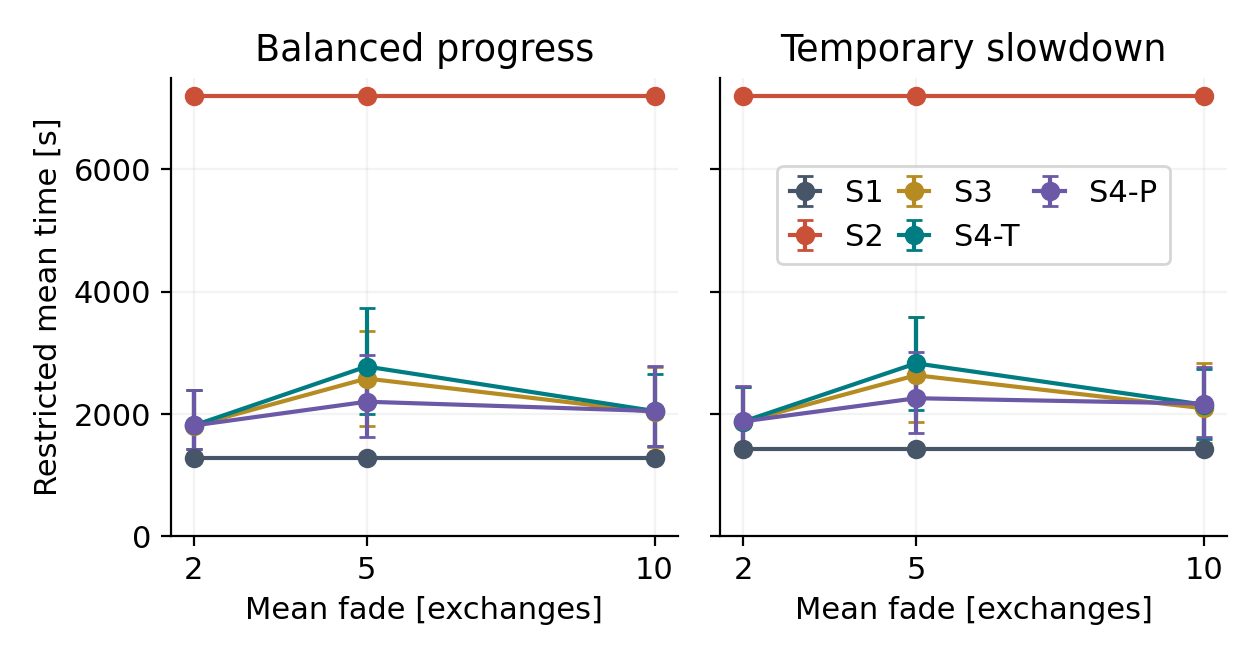
\includegraphics[width=\linewidth]{generated/mission-time.png}
\caption{Restricted mean time to coverage with 95\% bootstrap intervals. Unfinished missions contribute $7200$ s without being counted as completed. Each point uses 30 seeds.}\label{fig:time}\end{figure}
\begin{table}[htbp]\centering\caption{Restricted mean time in seconds, rounded for display.}\label{tab:times}
\begin{tabular}{llrrrrr}\toprule
Progress & $L$ & S1 & S2 & S3 & S4-T & S4-P\\\midrule
Balanced & 2 & 1280 & 7200 & 1811 & 1814 & 1814\\
Balanced & 5 & 1280 & 7200 & 2582 & 2778 & 2203\\
Balanced & 10 & 1280 & 7200 & 2030 & 2050 & 2050\\
Unequal & 2 & 1423 & 7200 & 1874 & 1878 & 1881\\
Unequal & 5 & 1423 & 7200 & 2635 & 2830 & 2260\\
Unequal & 10 & 1423 & 7200 & 2094 & 2153 & 2172\\
\bottomrule\end{tabular}

\end{table}
For balanced progress, S4-T minus S2 was $-5386$ s at $L=2$ (95\% interval $[-5773,-4810]$), $-4422$ s at $L=5$ ($[-5194,-3464]$), and $-5150$ s at $L=10$ ($[-5718,-4400]$). Under slowdown, the corresponding differences were $-5322$, $-4370$, and $-5047$ s. These restricted-time differences include S2's persistent non-completion. S1 remained faster than every online configuration in these settings, with means $1280$ s without slowdown and $1423$ s with slowdown.

\subsection{Reservation control and warning quality}
S4-T showed no consistent improvement over S3. Its mean restricted-time difference from S3 was positive in all six conditions, ranging from $2.8$ to $196.3$ s. At $L=5$ without slowdown it was $+196.3$ s ($[0.7,583.0]$); with slowdown it was $+194.2$ s ($[-0.2,577.5]$). The trend/persistence comparison was also mixed: at $L=5$ S4-T was about $575$ s slower without slowdown and $570$ s slower with slowdown, while several other conditions differed only slightly. The complete paired contrasts, including uncertainty, are provided with the generated data.

On held-out fixed-route replay, the trend predictor matched 197 of 757 eligible outages, with 1299 false alerts: precision $0.132$, recall $0.260$, F1 $0.175$. Persistence matched 196 outages with 1280 false alerts: precision $0.133$, recall $0.259$, F1 $0.176$. Forty early-boundary outages per predictor and 25 late-boundary alerts per predictor were excluded and counted. These scores do not indicate a substantial trend-predictor advantage.

\subsection{Coverage and resource trade-offs}
The online long-queue and predictive methods produced redundant observations, including travel through already observed cells; S2's zero redundancy accompanies severe incomplete coverage. No duplicate task ownership or session-budget violation was detected in the reconstructed evaluation logs. Communication attempts, bytes, component operation counts, idle time, and missing-information fractions are retained per run and summarized by condition. Counts stop at completion or timeout.
\begin{figure}[htbp]\centering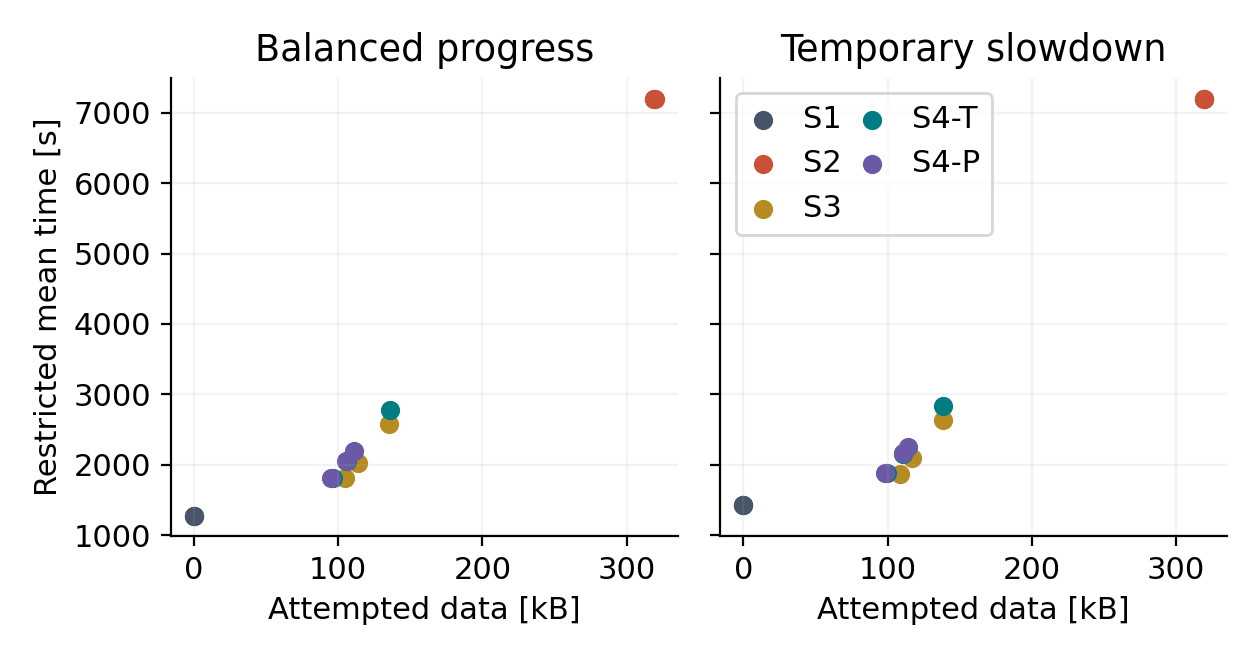
\includegraphics[width=\linewidth]{generated/resource-tradeoff.png}
\caption{Communication volume and restricted time, interpreted alongside completion and achieved coverage. Points represent conditions, not an imposed weighted score.}\end{figure}
\Needspace{12\baselineskip}
\begin{table}[htbp]\centering
\caption{Descriptive resource means over all 180 runs per policy, with six equally sized conditions, measured until completion or timeout. Low resource use in an incomplete mission is not efficiency. Missing-information gaps are averaged before synchronization.}
\begin{tabular}{lrrrr}\toprule
Policy & Attempted kB & Arithmetic ops & GOP & Mean gap [\%]\\\midrule
S1 & 0.0 & 0 & 0.000000 & 25.70\\
S2 & 319.3 & 229762 & 0.000230 & 1.62\\
S3 & 119.7 & 1932120 & 0.001932 & 1.21\\
S4-T & 114.6 & 1100751 & 0.001101 & 1.22\\
S4-P & 105.8 & 1004105 & 0.001004 & 1.10\\
\bottomrule\end{tabular}

\end{table}
\par Separate repeated saved-input benchmarks on the recorded host measured median CPU time per decision of 6.7 $\mu$s for trend, 1.4 $\mu$s for persistence, and 366.2 $\mu$s for the representative allocation. Isolated full-process peak RAM ranged from 41.6 to 43.2 MiB across the five configurations. These are implementation- and host-specific measurements. Incremental Python allocation profiles and all batch timings are retained separately; small per-session CPU counters may be below the Windows timer resolution.

